%%%%%%%%%%%%%%%%%%%%%%%%%%%%%%%%%%%%%%%%%
% Imperial College London Poster (Portrait)
% LaTeX Template
% Version 1.0 (February 22, 2024)
%
% For current versions and to report
% issues, please see:
% https://github.com/ImperialCollegeLondon/imperial_latex_templates
%
%!TEX program = xelatex
% Note: this template must be compiled with XeLaTeX rather than PDFLaTeX
% due to the custom fonts used. The line above should ensure this happens
% automatically, but if it doesn't, your LaTeX editor should have a simple toggle
% to switch to using XeLaTeX.
%
% © Imperial College London, 2024. This template, including logo and fonts, is 
% for use of Imperial staff and students only for university business. All rights 
% reserved to the copyright owners.
%
%%%%%%%%%%%%%%%%%%%%%%%%%%%%%%%%%%%%%%%%%

%----------------------------------------------------------------------------------------
%	CLASS, PACKAGES AND OTHER DOCUMENT CONFIGURATIONS
%----------------------------------------------------------------------------------------

\documentclass[
	%print, % Uncomment to convert colors to CMYK for printing purposes
	%a1papersize, % Uncomment to use an A1 paper size instead of the default A0 paper size
]{ImperialPoster}

%----------------------------------------------------------------------------------------
%	POSTER INFORMATION
%----------------------------------------------------------------------------------------

\postertitle{Title\\ Fully implicit moisture-dynamics coupling} % The poster title, can be split across multiple lines manually with \\

% Contributor/author names, can be split across multiple lines manually with \\
% Add affiliations using the \affiliation{} command
\posterauthors{Colin Cotter\affiliation{1}}

% Command to output coauthor logos to the right of the Imperial logo in the header of the poster
% If no coauthor logos are required, remove or comment out this command
\coauthorlogos{
  \coauthorlogo[4cm]{firedrake.png} % Use the optional parameter to specify a height for the logo
}

%----------------------------------------------------------------------------------------

\usepackage{biblatex}
\usepackage{setspace}
\setlength{\bibitemsep}{0pt}
\addbibresource{poster.bib}


\begin{document}

%----------------------------------------------------------------------------------------
%	EXAMPLE POSTER LAYOUT 1
%----------------------------------------------------------------------------------------

\titlesection % Output the title section, automatically populated using the information in the POSTER INFORMATION block above

\begin{multicols}{3} % Start the three-column layout
	
	%----------------------------------------------------------------------------------------
	%	FIRST COLUMN
	%----------------------------------------------------------------------------------------

   Instead of building complicated splitting methods between different
   dynamics and physics components, we consider applying implicit
   Runge-Kutta methods to the entire coupled system (moving the
   complexity to finding a good iterative solver). In NWP this
   requires reinterpretation of physics processes as terms in a
   differential equation. In particular, this has been made possible
   for some moisture parameterisations. Here we focus on the thermal
   rotating shallow water equations with moisture as an exploratory
   toy system, in particular the formulation of
   \cite{zerroukat2015moist} (see also, \cite{rostami2018improved}).

   All results are presented using Firedrake \cite{FiredrakeUserManual}
   and PETSc \cite{petsc-user-ref}.
   
  \section{Scalable monolithic solvers}

  A ``monolithic'' solver treats the full system of coupled variables
  without elimination. To solve the nonlinear algebraic system from an
  implicit Runge-Kutta method we use:
  \begin{itemize}[noitemsep, topsep=0pt]
  \item Nonlinear system solver: \emph{linesearch Newton},
  \item Jacobian solver (for $J$ evaluated at current Newton state):
    \emph{Preconditioned GMRES},
  \item Preconditioner: \emph{monolithic geometric multigrid (V cycle)},
  \item Multigrid smoothers: \emph{additive Schwarz method (ASM)}.
  \end{itemize}

  \subsection{ASM} The mesh is decomposed
  into overlapping patches, and the fully coupled Jacobian is solved
  independently (and hence parallelisably) on each patch. The result of the
  smoother is the sum of the solutions over all of the patches. In
  this work, a ``vertex star'' patch is used: it includes all of the
  degrees of freedom in the cells sharing one vertex, excluding those
  associated to the boundary (see Figure 1).

  \subsection{Solver performance: Linearisation about state of rest}
  For the rotating shallow water equations on the sphere linearised
  about a state of rest, the monolithic solver converges at a rate
  that is robust to mesh refinement and changes in $\Delta t$. Figure
  1 shows the average GMRES iterations per timestep to achieve a
  residual reduction of $10^{-10}$, using the ``Williamson 5
  mountain'' initial conditions and topography, run for 1 day. A
  compatible finite element discretisation with BDM2-DG1 spaces on
  triangles is used (3 pressure DOFs and 7.5 velocity DOFs per cell), with Crank-Nicholson
  implicit timestepping.

  \vspace{3mm}
  \begin{multicols}{2} 
    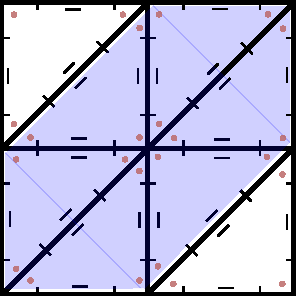
\includegraphics[width=10cm]{Images/patch}
\columnbreak
  \begin{tabular}{ccc}
    Cells & $\Delta t$ & GMRES its/step \\
    \hline
    20480 & 3600s & 8 \\
    81920 & 3600s & 8 \\
    327680 & 3600s & 8 \\
    20480 & 1800s & 8 \\
    20480 & 7200s & 8 \\
    20480 & 14400s & 8.6 \\
  \end{tabular} \\
  \end{multicols}
  \begin{center}
      \vspace{-8mm}
  {\bfseries Figure 1}: (LEFT) a diagram showing the ``vertex star'' patch. (RIGHT)
  iteration counts for the monolithic solver applied to the linear
  rotating shallow water equations on the sphere.
  \end{center}

  \subsection{Solver performance: linearisation about current state}
For the nonlinear rotating shallow water equations, the introduction
of advection terms degrades $\Delta t$ robustness but mesh independent
iteration counts are achieved upon maintaining a constant Courant
number (see Figure 2). BDM2-DG1 spaces on triangles are used
with Crank-Nicholson implicit timestepping.

  \begin{tabular}{cccc}
    Cells & $\Delta t$ & GMRES its/step & Wallclock \\
    \hline
    20480 & 3600s & 18.86 & T \\
    81920 & 1800s & 18.03 & T \\
    327680 & 900s & 18.00 & T \\
  \end{tabular} \\
  \begin{center}
      \vspace{-8mm} {\bfseries Figure 2}: Average number of GMRES
      iterations per timestep, and wallclock times, for nonlinear
      rotating shallow water equations running the ``Williamson 5
      mountain'' testcase until 15 days at various resolutions and
      fixed $\Delta x/\Delta t$ ratio, on 16 cores.
  \end{center}
  
\columnbreak


\cite{cotter2023compatible}

        \columnbreak

        
        
        \AtNextBibliography{\small}
        \printbibliography
        
	\subsection{Affiliations}
		
	% Affiliation institutions, the first parameter is the affiliation number (matching the author list) and the second is the institution
	\affiliationentry{1}{Department of Mathematics, Imperial College London}
	
	\subsection{Funders}
	
	
\includegraphics[width=0.55\linewidth]{UKRI_logo.png}\hfill
\includegraphics[width=0.35\linewidth]{Grey_16-9.pdf} % Side by side funder logos
	
%----------------------------------------------------------------------------------------

\end{multicols}

%----------------------------------------------------------------------------------------

\end{document}
